\documentclass[utf8,handout]{beamer}
\usepackage{presentation}
\title{Сервис поиска электронных книг }
\subtitle{Серверная часть, обеспечивающая верификацию, обновление данных и взаимодействие с клиентскими программами и пользователем.}
\author{Е. А. Тузова}

\institute{Академический Университет РАН}
\date{}


\begin{document}

\begin{frame}
  \titlepage

  \begin{flushright}
%    Студент~~~~~~  Е. А. Тузова
  
    Руководитель~~~  Н. М. Пульцин

  \end{flushright}
\end{frame}


\begin{frame}
	\frametitle{Место в общей системе}
	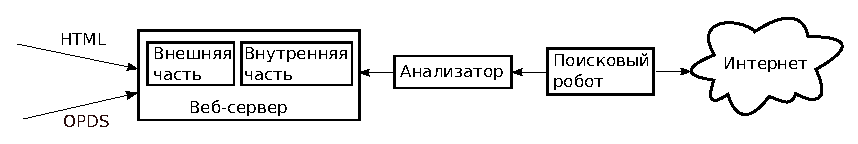
\includegraphics[width=1.05\textwidth]{./head/innerstructure-new}
\end{frame}

\section*{План}
  \begin{frame}
    \frametitle{План}
    \tableofcontents[pausesections]

  \end{frame}

\section{Протокол OPDS}
  \begin{frame}
    \frametitle{Протокол OPDS}
    \begin{block}{}
	OPDS (The Open Publication Distribution System) - стандарт для предоставления информации об электронных документах, построенный на базе протокола публикации Atom.
	\end{block}
	\ 
    
	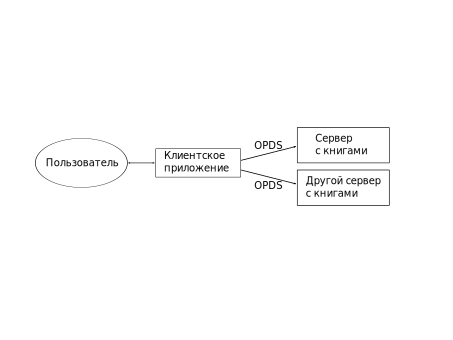
\includegraphics{./head/scheme}
  \end{frame}

\section{Постановка задачи}
  \begin{frame}

    \frametitle{Постановка задачи}
    \begin{enumerate}
      \item Предоставление данных пользователю и клиентским программам
      \item Верификация и обновление данных
    \end{enumerate}
  \end{frame}

\section{Предоставление данных}
  \begin{frame}
    \frametitle{Предоставление данных пользователю и клиентским программам}  
    
	\begin{itemize}
      \item Абстракция MVC(Model-View-Controller) в Django
      \item Форматы предоставления информации
          \begin{itemize}
            \item xHTML
            \item OPDS
          \end{itemize}        

    \end{itemize}        
    
  \end{frame}



\section{Задача верификации и обновления данных}
  \begin{frame}
    \frametitle{Задача верификации и обновления данных}
  
    Верификация:
    \begin{itemize}
      \item Интерфейс администратора
    \end{itemize}

    \ 
    
  	Обновление:
    \begin{itemize}
      \item Извлечение информации из форматов epub и fb2 
      \item Поиск информации на внешних ресурсах
      \item Определение жанра книги
    \end{itemize}

  \end{frame}
  

\section{Определение жанра книги}
  \begin{frame}
    \frametitle{Определение жанра книги}  
    
    \begin{itemize}
      \item Деревья принятия решений
      \item Метод k-средних
      \item Нейронные сети
		
	  \ 
		
      \item Байесовский классификатор
    \end{itemize}        
  \end{frame}

\begin{frame}
	\frametitle{Байесовский классификатор}
	  \begin{itemize}
	    \item Возможность инкрементального обучения
	    \item Простота интерпретации
	    \item Простые математические операции
	  \end{itemize}
	   		  
\end{frame}


\begin{frame}
	\frametitle{Алгоритм}
      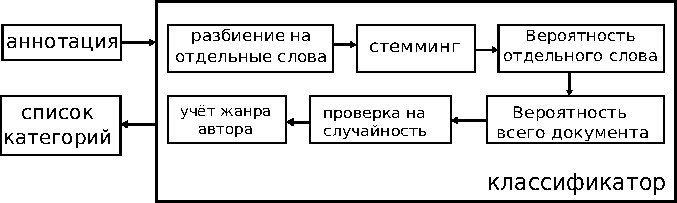
\includegraphics[width=1.05\textwidth]{./classifier}
\end{frame}

\begin{frame}
	\frametitle{Статистика}
   \begin{figure}
	  \centering
	  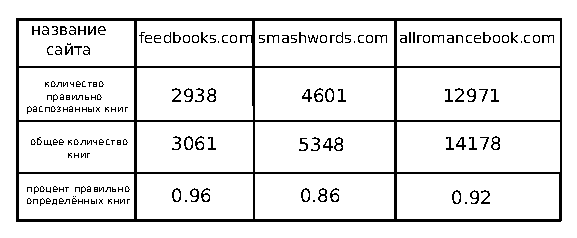
\includegraphics[width=.7\textwidth]{./statistics}
	  
	  \ 
	  \ 
	  
	  Таблица успешности распознавания жанра книги.
   \end{figure} 
\end{frame}


\section{Заключение}
  \begin{frame}
    \frametitle{Заключение}
    \begin{enumerate}
      \item Реализовано предоставление данных в xHTML виде для пользователей и по протоколу OPDS для клиентских программ	  
	  \item Усовершенствован стандартный интерфейс администратора, предоставляемый фреймворком Django.
	  \item Реализован поиск дополнительной информации и извлечение информации из форматов ePub и FB2
      \item Для обновления информации реализован самообучающийся классификатор, позволяющий предсказать жанр книги по её аннотации.
	  
    \end{enumerate}
  \end{frame}

\end{document}